\documentclass{article}
\usepackage{amsmath}
\usepackage{hyperref}
\usepackage{graphicx}
\newcommand{\tabincell}[2]{\begin{tabular}{@{}#1@{}}#2\end{tabular}}

\begin{document}
\begin{titlepage}
\title{EE 239AS \\Special Topics in Signals and Systems\\Project 3\\Collaborative Filtering\\Winter 2016} 
\author{Liqiang YU, Kaiming WANG and Jun FENG\\
904592975, 504592374, 304588434} 
\date{03-04-2016}
\end{titlepage}

\maketitle
\newpage
\tableofcontents
\newpage
\section{Introduction}
In this project, we tried to build a movie recommendation system based on the collaborative filtering algorithm. This method based on the fact that there existed some other users who has the similar behaviors so we can use them to make the prediction for a specific target user. First some data preprocessing steps were taken to create the rating matrix. Then we implemented different matrix factorization algorithms to retrieve two factor matrices and get the prediction matrix. The prediction result were measured with 10-fold cross validation and the trade off curve between precision and recall. Finally, we evaluated the effect of our recommendation system by changing the number of movies we want to recommend.\\
\\
The report is organized as follows: In section 1, we introduce the dataset we use briefly and weighted non-negative matrix factoration to predict missing data. In section 2, we use cross-validation technique. In section 3, we try to sweep threshold of predicted data in a binary classification problem to find out the relation between precision and recall.
%\section{Dataset  \& Weighted Non-Negative Matrix Factorization}
\section{Data Preprocessing}
In this project, we use MovieLens data sets, which were collected by the GroupLens Research Project at the University of Minnesota. This data set consists of 100,000 ratings from 1 to 5 from 943 users on 1682 movies. So we use the Import Data tool of MATLAB to transfer raw data file into a 100,000*4 matrix and four columns are userId, itemId, rating and timestamp, respectively. Use the first three columns, we can achieve a 943*1682 matrix $R$, $R(i,j)$ represent rating of user $i$ on item $j$.

\section{Weighted Non-Negative Matrix Factorization}
Since we only have 100,000 ratings in the data sets, there are many missing ratings in matrix $R$, which is fulfilled by NaN values. In order to predict these values, we can employ non-negative matrix factorization to get matrices $U, V$ such that $R_{m \times n}=U_{m \times k}V_{k \times n}$. It is necessary to calculate the least square error and minimize it.\\
\\
This can be implemented by putting 0s where the data is missing and creating a weight matrix to calculate the squared error. Assume that the weight matrix $W_{m \times n}$ contains 1 in entries where we have known data points and 0 in entries where the data is missing. At last, we can formulate the above problem as:
\begin{equation*}
min\sum_{i=1}^{m}\sum_{j=1}^{n}w_{ij}{(r_{ij}-{(UV)}_{ij})}^2
\end{equation*}
\\
Luckily, we do not need to implement this factorization by hand. Instead, we can use \emph{wnmfrule} function in the Matrix Factorization Toolbox in MATLAB. By choosing the $k$ equal to $10, 50, 100$, the total least squared error is shown in table \ref{tb:k}.
\begin{table}
\begin{center}
\caption{The least square error with different K}
\label{tb:k}
\begin{tabular}{|c|c|c|c|}
\hline
k& 10& 50 & 100\\
\hline
least square error&54466.7386&19425.539&6202.9535\\
\hline
\end{tabular}
\end{center}
\end{table}
\subsection{10-fold Cross-validation}
As before, we will use cross-validation in our recommendation system design. We will divide 100,000 records into 10 folds exclusively. Each time, we use 9 folds as trainset and remaining 1 fold as testset. However, we will calculate average absolute error over testing data among all entries this time, not previous total least squared error as in section 1.
\begin{itemize}
\item Average absolute error over testing data for each entry of all 10 tests is \emph{233.9302}.
\item Highest average absolute error over testing data for each entry is \emph{1696.0535}.
\item Lowest average absolute error over testing data for each entry is \emph{1.1073}.
\end{itemize}
However, among 10 tests, the average absolate error of most of them are below 2, while the average absolate error of the remaining two or three tests are very high.
\subsection{Precision Over Recall}
According to testing data, we can assume that if a user has rated a movie 3 or lower we conclude they didn't like the movie, and if a user has rated a movie 4 or higher they have liked it. However, when it comes to predicted data, it is our job to set the threshold to decide whether users like or dislike items.\\
\\
Out of all predicted entries in which user likes the item, the percentage of the user actually like the item is precision. While out of all entries in which user actually likes the item, the percentage entries which we have predicted successfully is recall.\\
\\
In figure \ref{fig:problem3}, we plot the curve of precision versus recall. We can find that there is a tradeoff between precision and recall at most time. And the area under this curve is $0.64685$
\begin{figure}[htbp]
\centering
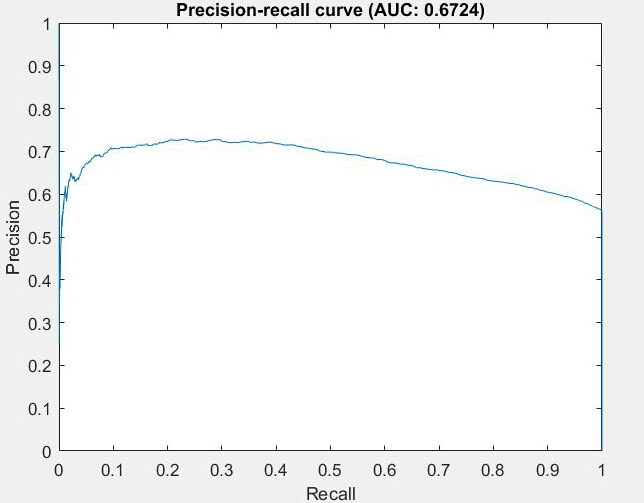
\includegraphics[width=.6\textwidth]{problem3.jpg}
\caption{Precision versus Recall}
\label{fig:problem3}
\end{figure}

\section{Weighted Non-Negative Matrix Factorization with Regularization}
In the previous section, we talked about how to make recommendation based on the weighted non-negative matrix factorization. In this part, we replaced rating matrix with weight matrix and vice versa. The total square error was reduced to ???. However without any regularization parameter, the prediction matrix would all be 1. Therefore, we add some regularization parameters to the cost function. The new version cost function is as follow:
\begin{equation*}
min\sum_{i=1}^{m}\sum_{j=1}^{n}w_{ij}{(r_{ij}-{(UV)}_{ij})}^2 + \lambda\left( \sum_{i=1}^m\sum_{j=1}^ku_{ij}^2+\sum_{i=1}^k\sum_{j=1}^nv_{ij}^2\right) 
\end{equation*}
\subsection{Regularized Version of Alternating Least Squares}
In the alternating least squares algorithm that is implemented in many recommendation system, we need to construct a binary matrix P
\begin{equation*}
P = \begin{cases}
				1, R > 0\\
				0, R = 0
		\end{cases}
\end{equation*}
Then we want to factorize P into X and Y such that $P \approx XY^T$. The recommendations are largest values in $XY^T$. Since optimizing X and Y simultaneously is non-convex, alternating least squares idea was used, for the reason that if X or Y is fixed, it's just a system of linear equations, which is convex and easy to solve. The solving processes are as follows:
\begin{enumerate}
\item Initialize Y with random values
\item Solve for X
\item Fix X, solve for Y
\item Repeat above processes until it converges
\end{enumerate}
Let's define the regularization weights $c_{ui} = r_{ui}$, where the subscripts are for user $u$ and movie $i$, and define $C_u$ as the diagonal matrix of $c_u$. Then the update equation for x is
\begin{equation*}
x_u = (Y^TC_uY+\lambda I)^{-1}Y^TC_up_u
\end{equation*}
\subsection{Evaluation of the Results}
We used the same evaluation methods to test the result of the regularized ALS. The total least square error with different $\lambda$ is shown in table \ref{tb:lamda}. Compared with the results in the previous part, we can see that the errors were reduced. The precision VS recall curve is shown in figure ??? and the area under curve is ???. When setting the threshold to 3, the precision is ??? and the recall is ???.
\begin{table}
\begin{center}
\caption{The least square error with different $\lambda$}
\label{tb:lamda}
\begin{tabular}{|c|c|c|c|}
\hline
$\lambda$& 0.01& 0.1 & 1\\
\hline
least square error&???&???&???\\
\hline
\end{tabular}
\end{center}
\end{table}
\section{Creating the Recommendation System}
The precision of our recommendation system depended on the prediction matrix P and how many movies you want to recommend. When choosing top 5 movies, the precision in the 10-fold cross validation is shown in figure \ref{fig:p5} and the average precision is 84.07\%.\\
\\
\begin{figure}[htbp]
\centering
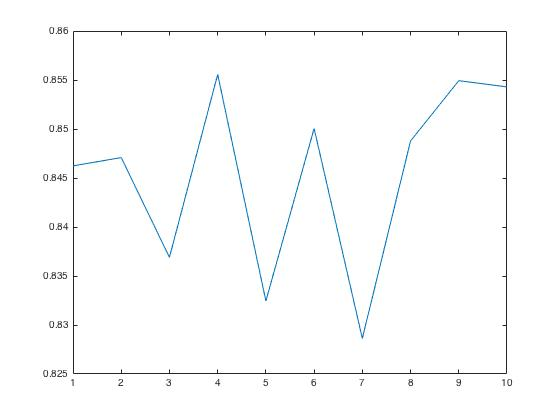
\includegraphics[width=.6\textwidth]{precision_5.jpg}
\caption{The precision over 10-fold cross validation}
\label{fig:p5}
\end{figure}
The hit rate and false alarm rate can change dramatically with different number of recommendations. The results is shown in figure \ref{fig:hit}. From the figure we can see, at the beginning the hit rate increased dramatically with the increasing of the recommendations. After some point, the false alarm rate increased more rapidly than the hit rate, which means the number of recommendation may not be larger than 20.
\begin{figure}[htbp]
\centering
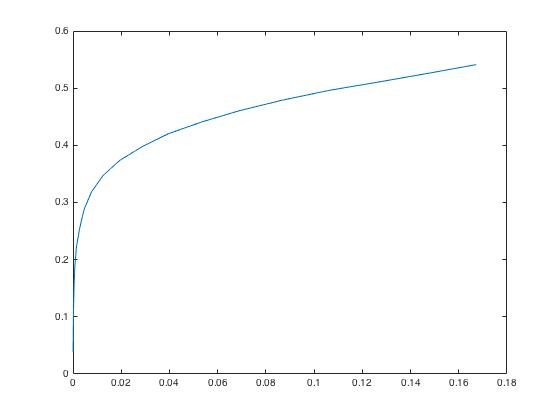
\includegraphics[width=.6\textwidth]{hit_false_20.jpg}
\caption{Hit rate VS false alarm rate}
\label{fig:hit}
\end{figure}


\end{document}

